\documentclass{article}
\usepackage[utf8x]{inputenc}
\usepackage{lipsum}
\usepackage[margin=1in,includefoot]{geometry}
\usepackage{pifont}
\newcommand{\cmark}{\ding{51}}
\newcommand{\xmark}{\ding{55}}
\usepackage{fancyhdr}
\pagestyle{fancy}
\usepackage{listings}
\usepackage{color}
\usepackage{hyperref}
\usepackage[table]{xcolor}
\usepackage{graphicx}
\usepackage{float}
\usepackage{longtable}
\usepackage[T1]{fontenc}
\usepackage{textcomp}
\usepackage[english]{babel}
\usepackage[T1]{fontenc}
\usepackage{uarial}
\definecolor{delim}{RGB}{20,105,176}
\colorlet{numb}{magenta!60!black}
\renewcommand{\familydefault}{\sfdefault}
\colorlet{punct}{red!60!black}
\definecolor{dkgreen}{rgb}{0,0.6,0}
\definecolor{gray}{rgb}{0.5,0.5,0.5}
\definecolor{mauve}{rgb}{0.58,0,0.82}
\hypersetup{
    colorlinks=true, % make the links colored
    linkcolor=black, % color TOC links in blue
    urlcolor=blue, % color URLs in red
    linktoc=all % 'all' will create links for everything in the TOC
}
\definecolor{background}{HTML}{EEEEEE}
\lstset{
    commentstyle = \color{gray},
    extendedchars = \true,
    inputencoding = utf8x,
    language = php,
    keepspaces = true,
    keywordstyle = \bfseries,
    backgroundcolor = \color{blue!25},
    xleftmargin = 2cm,
    framexleftmargin = 1em
}
\lstdefinelanguage{json}{
    basicstyle=\normalfont\ttfamily,
    numbers=left,
    numberstyle=\scriptsize,
    stepnumber=1,
    numbersep=8pt,
    showstringspaces=false,
    breaklines=true,
    frame=lines,
    backgroundcolor=\color{background},
    literate=
     *{0}{{{\color{numb}0}}}{1}
      {1}{{{\color{numb}1}}}{1}
      {2}{{{\color{numb}2}}}{1}
      {3}{{{\color{numb}3}}}{1}
      {4}{{{\color{numb}4}}}{1}
      {5}{{{\color{numb}5}}}{1}
      {6}{{{\color{numb}6}}}{1}
      {7}{{{\color{numb}7}}}{1}
      {8}{{{\color{numb}8}}}{1}
      {9}{{{\color{numb}9}}}{1}
      {:}{{{\color{punct}{:}}}}{1}
      {,}{{{\color{punct}{,}}}}{1}
      {\{}{{{\color{delim}{\{}}}}{1}
      {\}}{{{\color{delim}{\}}}}}{1}
      {[}{{{\color{delim}{[}}}}{1}
      {]}{{{\color{delim}{]}}}}{1},
}
\begin{document}
\rowcolors{2}{teal!20}{white}
\begin{titlepage}
\begin{center}
\begin{figure}[H]
\centering


\includegraphics[width=0.8\textwidth]{306.png}
\end{figure}
\line(1,0){350}\\
\huge{\bfseries Zaakpay Link Based Payments}
\line(1,0){250}\\
[1.5cm]
\textsc{\Large Version 2.0}
\end{center}
\end{titlepage}
\thispagestyle{empty}
\tableofcontents
\thispagestyle{empty}
\newpage
\thispagestyle{empty}
\cleardoublepage
\setcounter{page}{1}
\section{Introduction}
\begin{itemize}
\item This feature enables merchant's to share payment links to their customers. This link redirects the users to the gateway page where they can complete the payments.
\item Once the payment is complete, the merchant can call the check API to confirm the status of the transaction.
\item The URL to this interface is  {\bfseries https://api.zaakpay.com/invoicePayment.jsp}\\
\item Below is the interface of the link based payment solution.
\end{itemize}
\begin{figure}[H]
\centering
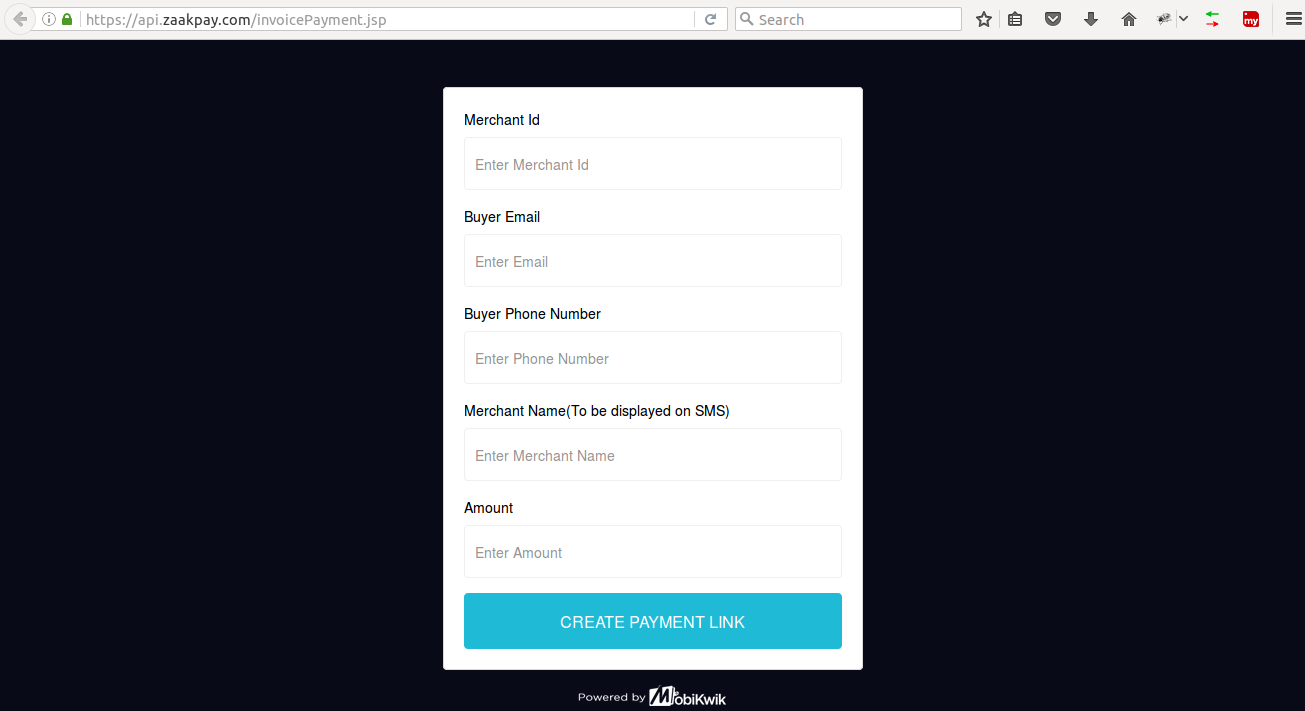
\includegraphics[width=7.4in]{invoicepage.png}
\end{figure}
\newpage
Below is the list of fields required to generate the link as per the screen above:
\begin{itemize}
\item Merchant ID: We will be providing you a separate merchant ID which will be static for a merchant
\item Buyer Email: Email address of the customer
\item Buyer Phone number
\item Amount : This is the amount that is to be debited from the customer's account. This amount will be in Rupees
\item Merchant Name : A specific name to be shown in the SMS
\end{itemize}
The above page will call the API returning the status of the SMS
having the link to payment.
\\ The SMS to the customer would look like 
\begin{figure}[H]
\centering
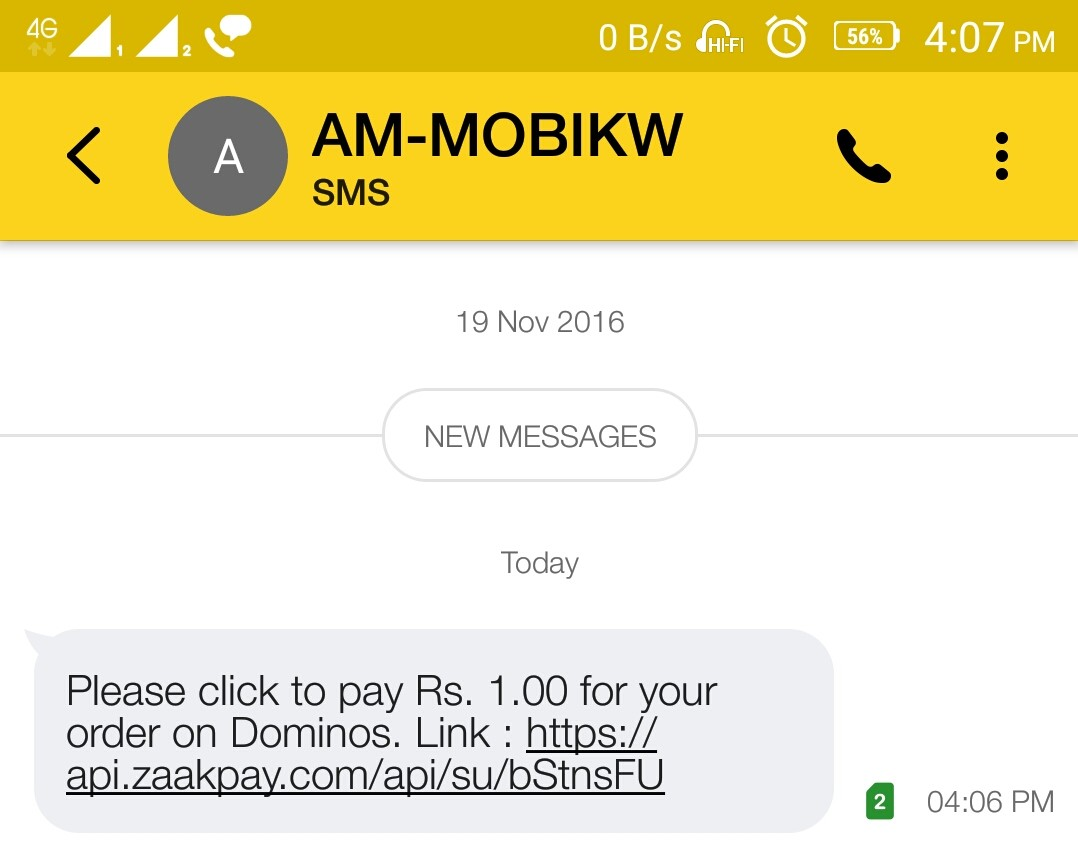
\includegraphics[scale=0.3]{Screenshot_2016-11-23-16-07-57-015.jpg}
\end{figure}
\newpage
\begin{itemize}
\item When user clicks on the link, they are redirected to the PG page where they have all the payment options available as shown below
\end{itemize}
\begin{figure}[H]
\centering
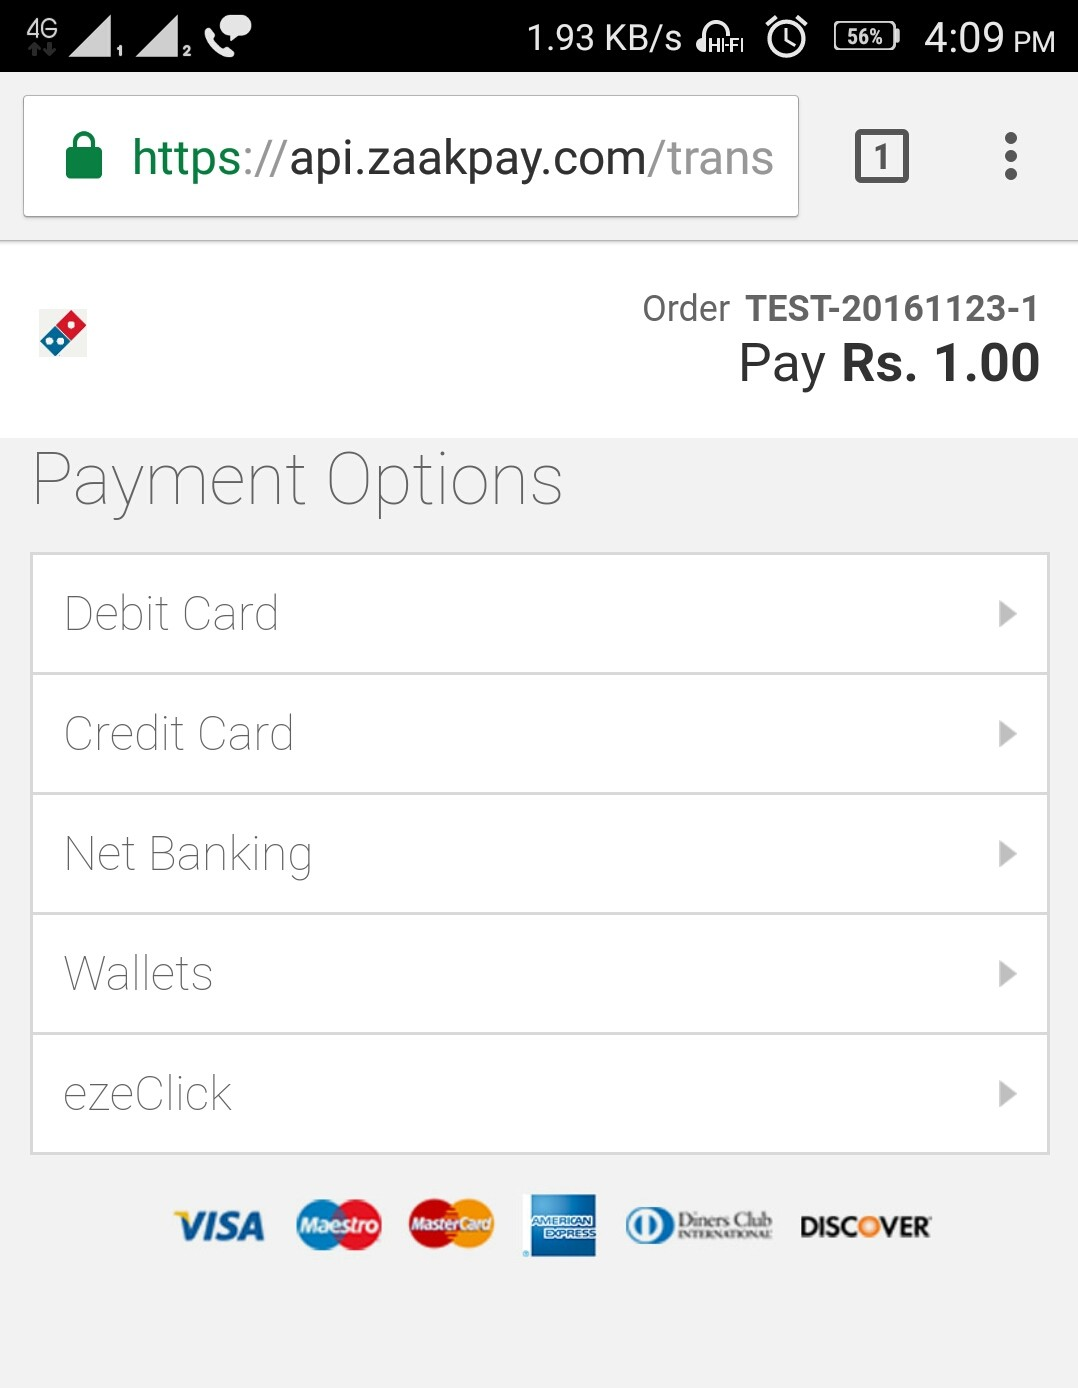
\includegraphics[scale=0.16]{Screenshot_2016-11-23-16-09-06-454.jpg}
\end{figure}
\begin{itemize}
\item User can select any of the payment options to complete the transaction as below :
\end{itemize}
\begin{figure}[H]
\centering
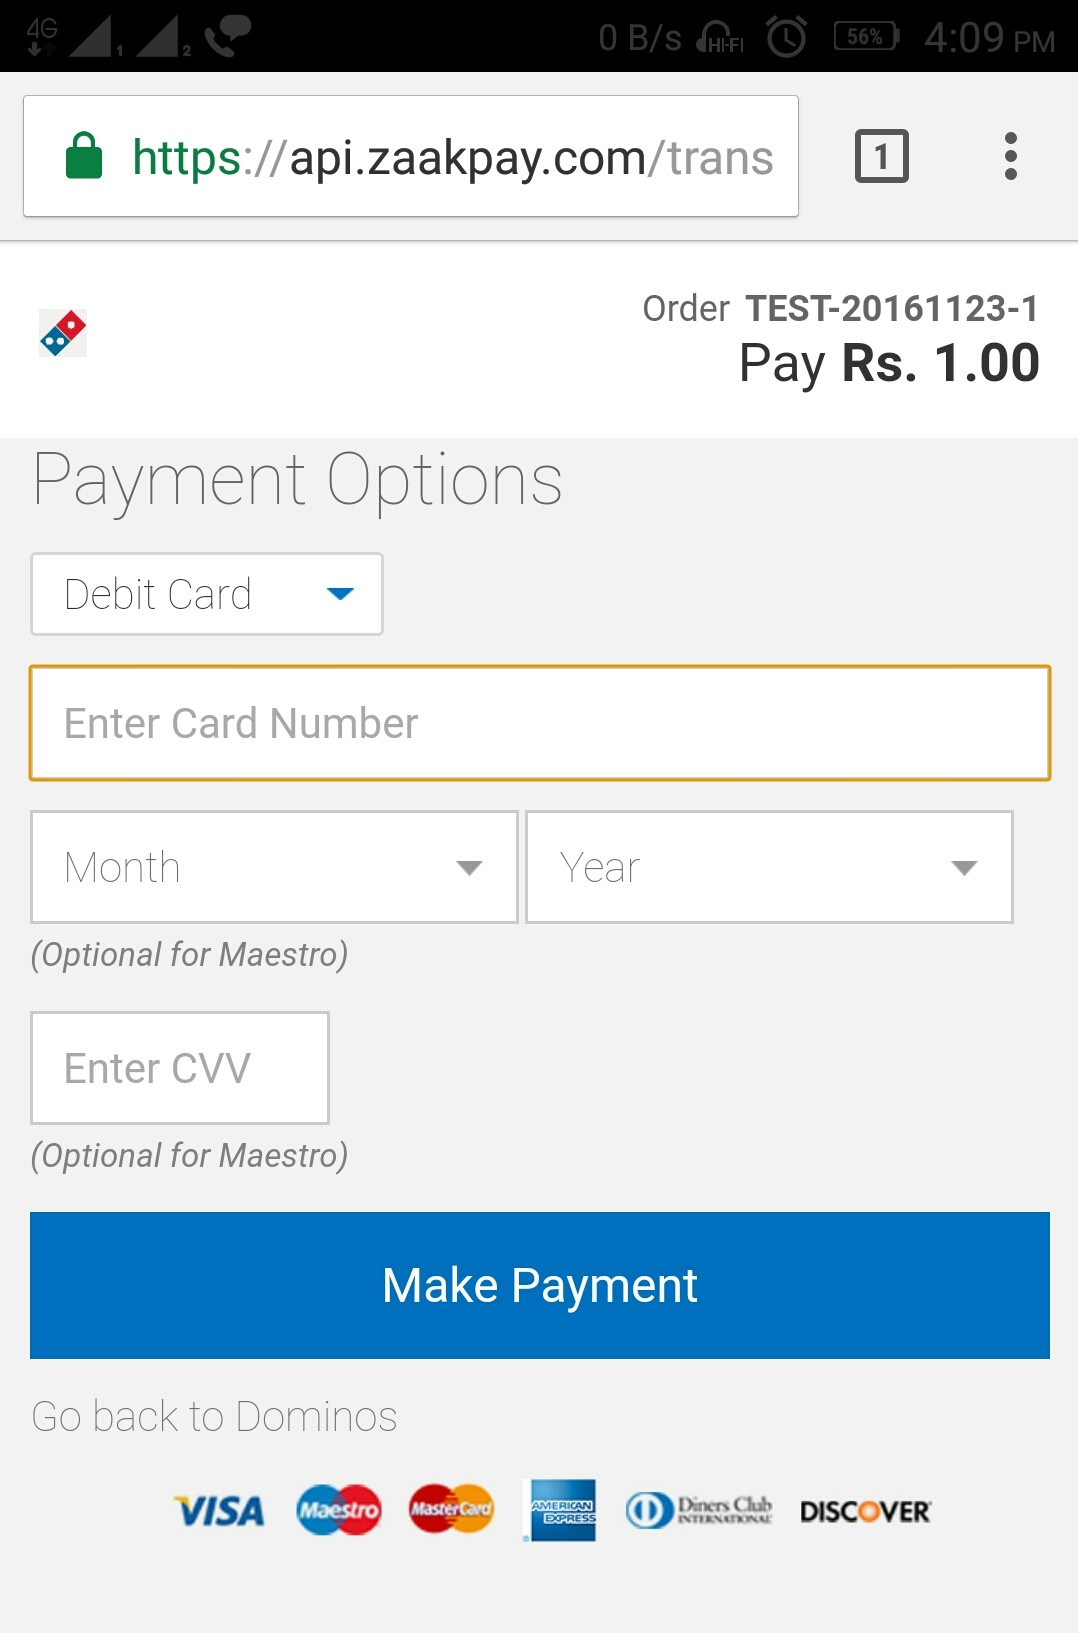
\includegraphics[scale=0.16]{Screenshot_2016-11-23-16-09-36-673.jpg}
\end{figure}
\begin{itemize}
\item 
\item Once the transaction is complete, the user is redirected to this page and the merchant will be getting a call-back if you have configured the URL in your Zaakpay profile.
\end{itemize}
\begin{figure}[H]
\centering
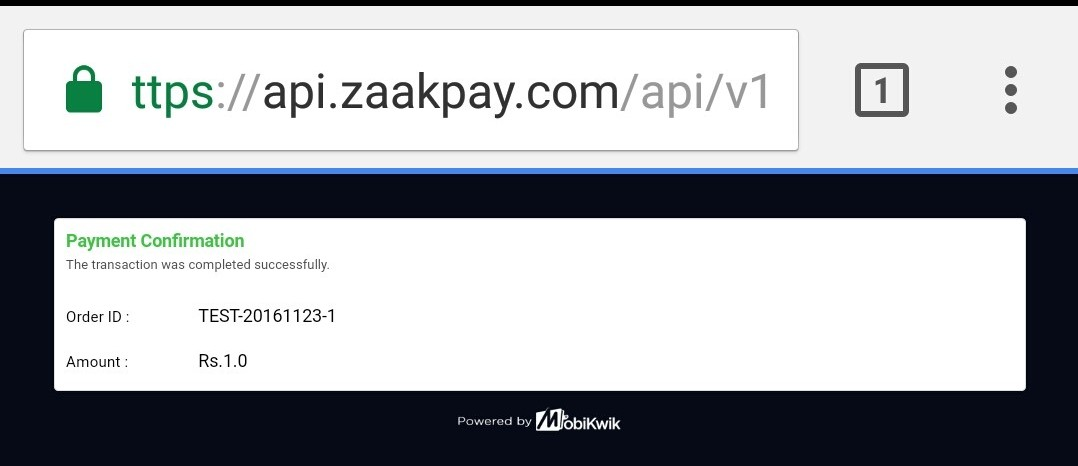
\includegraphics[width=17cm]{Screenshot_2016-11-23-16-10-28-991.jpg}
\end{figure}
\newpage
\section{API Flow}
URL for staging environment : 
{\bfseries http://zaakpay-staging.cloudapp.net:8080  } \\ \\
URL for production environment :
{\bfseries https://api.zaakpay.com } \\ \\
API URL - {\bfseries \{SERVER\}/api/v1/generatePaymentLink }
\\

 This will be a POST call to Zaakpay server along with the parameters described below :
 
\begin{lstlisting}[language=java,breaklines=true]
loginid //707 is the value for staging environment. Consult your respective account manager for production value
buyerEmail //you can pass store id here provided by your store; or pass users email id if available
buyerPhoneNumber //Pass users phone number here(maximum 15 characters)
orderId=INV1468410370380 //generate a random orderid or take orderid from merchant
returnUrl={SERVER}/api/v1/getInvoiceResponse
showMobile=DETECT
buyerFirstName //User's detail
buyerLastName //User's detail
buyerAddress //User's detail
buyerCity //User's detail
buyerState //User's detail
buyerCountry //User's detail
buyerPincode //User's detail
txnType=1
zpPayOption=1
mode=0
currency=INR
zpAmount // eg. 12300 Pass amount in paisa e.g: 100 for 1rupee
amount // eg. 12300 Pass amount in paisa e.g: 100 for 1rupee
merchantIpAddress // IP address of your website
purpose=4
productDescription //eg. Invoice+Payments
product1Description //
shipToAddress //User's detail
shipToCity //User's detail
shipToState //User's detail
shipToCountry //User's detail
shipToPincode //User's detail
shipToPhoneNumber //User's detail
shipToFirstname //User's detail
shipToLastname//User's detail
txnDate= // eg. 2016-7- 13 ,pass correct date in the specified format
\end{lstlisting}
\newpage
This will be a server to server call. The response of this API would be :
\begin{lstlisting}[language=json,breaklines=true]

{
       "status":100,     // 100 for success, others for failure
      "message":"Success"
}
\end{lstlisting}
\section{Checksum Calculation for response}
For both integrity \& data-authenticity verification before sending data to the API, you need to calculate a checksum of all the data that you send to Zaakpay. We use an HMACSHA- 256algorithm to calculate the checksum of ALL data that is posted to the API. We require data to be posted to our server in NVP (Name- Value Pairs) format. \\
To calculate the checksum please follow the process below:
\begin{itemize}
\item Create a list of all parameters which you’re passing to the API. Parameters used in checksum calculation are in the same order as the order of posting the parameters to Zaakpay
\item Create a concatenated string of all data values in your list, with single quotes around each item. e.g.
'merchantIdentifier''orderId''amount''buyerEmail''buyerAddress'...
\item Calculate the checksum using the HMAC SHA-256 algorithm using the concatenated string as data
and your generated secret key
\item The resulting checksum calculated should be posted to the Zaakpay API along with other data. For
example: Let’s suppose we need to post the following data to the API. We calculate "checksum" only with the parameters mentioned below and the order of the parameters must remain intact when calculating "checksum"
\begin{itemize}
\item merchantIdentifier -b19e8f103bce406cbd
\item orderId –223453
\item mode -1
\item merchantIpAddress –10.45.46.127
\item txnDate –2014-09-22
\end{itemize}
\item Now, we have to create a concatenated string of all the values, in the order in which they’ll be sent to the API, with single quotes around each item. The string therefore will be: \\
'b19e8f103bce406cbd''223453''1''INR''20000''10.45.46.127''2013-05-23'\\
Now you can calculate the checksum based on this concatenated string and the secret key generated in your account under the URLs \& Keys tab.
\end{itemize} \newpage
\section{Check API}
The purpose of this API is to enable websites to check the latest status of their transaction at any time.
Check status URL: {\bfseries https://api.zaakpay.com/checktransaction?v=2}
\subsection{Request Parameters}
\begin{longtable}{||c| p{2.09cm}| p{5.5cm}| p{4.7cm}||}
\rowcolor{white}
\caption{Check API Request}\\
   \rowcolor{green!50}
\bfseries{Parameter} & \bfseries{Optional O, Mandatory M} & \bfseries{Validation} & \bfseries{Allowed Values} \\ \hline
&&&\\
merchantIdentifier & M & alphanumeric &  \\
orderId & M & Transaction id for which you want to check the status & Your unique transaction identifier\\
mode & M & 1 digit only, numeric & 0\\
checksum & M & Checksum calculated on all above request parameters & \\
\end{longtable}

The parameters must be posted to the Update Transaction API using HTTP(POST). Apart from the listed parameters, a checksum is also expected. Refer below section for clarification on checksum generation.
\\

 Checksum Calculation: \\
Create a list of all parameters which you're passing to the API. Parameters used in checksum calculation are (in no particular order):\\
\begin{itemize}
\item merchantIdentifier
\item mode
\item orderId
\end{itemize}

Create a concatenated string of all data values in your list, with single quotes around each item. \\
Calculate the checksum using the HMAC SHA-256 algorithm using the concatenated string as data and your generated secret key.\\
The resulting checksum calculated should be posted to the Zaakpay API along with other data.For example: Let's suppose we need to post the following data to the API.We calculate "checksum" with the parameters mentioned below:\\
\begin{itemize}
\item merchantIdentifier -b19e8f103bce406cbd
\item mode - 0
\item orderId - ZPK12345
\end{itemize}

Now, we have to create a concatenated string of all the values, in the order in which they'll be sent to the API, with single quotes around each item. The string therefore will be: \\
{\bfseries \textquotesingle{}b19e8f103bce406cbd\textquotesingle{}\textquotesingle{}0\textquotesingle{}\textquotesingle{}ZPK12345\textquotesingle{}} \\
Now you can calculate the checksum based on this concatenated string and the secret key
generated in your account under the URLs \& Keys tab.\\
Example: \\
\begin{lstlisting}[language=html,breaklines=true]

<form action="https://api.zaakpay.com/checktransaction?v=2" method="post">
<input type="hidden" name="merchantIdentifier" value=”sk4jfdb342kjwdbkj9" />
<input type="hidden" name="orderId" value="897698973" />
<input type=”hidden” name=”mode” value=”0” />
<input type=”hidden” name=”checksum” value=”e2d9328528939568cc252e45aadb8” />
</form>
\end{lstlisting}

\subsection{Response Parameters}
The response will be in the XML format.
\begin{longtable}{||c|p{12.5cm}||}
     \caption{Check API Response}\\
 \rowcolor{green!50}
\bfseries{Parameters} & \bfseries{Description} \\ \hline
 & \\
merchantid & Zaakpay's unique identifier for your website \\
orderid & Your unique transaction identifier\\
responsecode &Numeric, max 3 digits example 100 for success \\
description &Alphanumeric max 30 description of the response \\
paymentmethod & Payment Method ID for Card and Net Banking transactions. For Card txns,payment Method ID starts with C and N for Net Banking. It is alphanumeric value with max length 6. First letter is C or N, followed by 5
digits max. \\
cardhashid &Unique id for each card number used in transaction. For Netbanking txns,value will be “NA”. \\
amount &Txn amount in paisa, Integer \\
checksum &Checksum calculated by Zaakpay on all above response parameters \\



\end{longtable}

Example:

\begin{lstlisting}[language=xml,breaklines=true]

<zaakpay_response>
<response_element>
<merchantid>sk4jfdb342kjwdbkj9</merchantid>
<orderid>99802312</orderid>
<responsecode>190</responsecode>
<description>OrderId either not Processed or Rejected</description>
<paymentmethod>NOT FOUND</paymentmethod>
<cardhashid>NA</cardhashid>
<amount>25000</amount>
<checksum>yun863a2d9328528939568cc252e45aadb8< /checksum>
</response_element>
</zaakpay_response>
\end{lstlisting}

\newpage
\section{Update API}
The purpose of this API is to enable websites to settle, cancel or refund transactions.
Update API URL: {\bfseries https://api.zaakpay.com/updatetransaction}
\subsection{Request Parameters}

\begin{longtable}{||c| p{2.09cm}| p{5.5cm}| p{4.7cm}||}
\rowcolor{white}
    \caption{Update API Request}\\
\rowcolor{green!50}
\bfseries{Parameter} & \bfseries{Optional O, Mandatory M} & \bfseries{Validation} & \bfseries{Allowed Values} \\ \hline
&&&\\
merchantIdentifier & M & alphanumeric & Zaakpay unique
merchant identifier for your website \\
orderId & M & Max 20 alphanumeric, must be unique per
website, we do not accept duplicate & Your unique transaction identifier\\
mode & M & 1 digit only, numeric & 0\\
updateDesired & M & Numeric max1digit, values predefined by Zaakpay & 7="Captured", 8="Canceled", 14="Refunded", 22=”Partial Refund”. Note:If you request a state update to "Refunded"we will issue the full amount refund to the user.\\
updateReason & M & Description of the reason for update. min5, max 50 alphanumeric characters. no special characters or dashes & Examples: you want to cancel a transaction, your user wants a refund, you want to settle a transaction \\
amount & O(during Full-Refund),M(for Partial-Refund) & Amount in paisa. Amount which needs to be refunded in case of partial refunds. In case of full refund this can be omitted. & example Re1 is 100 paisa, Rs 777.50 is 77750 paisa. Pass this parameter if merchant wants partial refund.\\
checksum & M & Checksum calculated on all above request parameters & \\
\end{longtable}

The parameters may be posted to the Update Transaction API using HTTP(POST). Apart from the listed parameters, a checksum is also expected. Refer below section for clarification on checksum generation.

Create a list of all parameters which you're passing to the API.Parameters used in checksum calculation are(in no particular order):

\begin{itemize}
\item merchantIdentifier
\item updateDesired
\item updateReason
\item orderId
\item mode
\end{itemize}

Create a concatenated string of all data values in your list, with single quotes around each item. \\
Calculate the checksum using the HMAC SHA-256 algorithm using the concatenated string as data and your generated secret key.\\
The resulting checksum calculated should be posted to the Zaakpay API along with other data.\\
For example: Let's suppose we need to post the following data to the API. We calculate "checksum" with the parameters mentioned below:\\
\begin{itemize}
\item merchantIdentifier - b19e8f103bce406cbd
\item updateDesired - 7
\item updateReason - Test Reason
\item orderId - ZPK12345
\item Mode - 0
\end{itemize}

Now, we have to create a concatenated string of all the values, in the order in which they'll be sent to the API, with single quotes around each item. The string therefore will be:\\
{\bfseries \textquotesingle{}b19e8f103bce406cbd\textquotesingle{}\textquotesingle{}7\textquotesingle{}\textquotesingle{}Test Reason\textquotesingle{}\textquotesingle{}ZPK12345\textquotesingle{}\textquotesingle{}0\textquotesingle{}} \\
Now you can calculate the checksum based on this concatenated string and the secret key
generated in your account under the URLs \& Keys tab. \\

{\bfseries Note}: \\
Only 3 kinds of updates are possible using Update API:\\
\begin{itemize}
\item Authorized to Cancel
\item Authorized to Capture
\item Capture to Refund before Payout Initiated
\item Capture to Partial Refund before Payout Initiated
\item Payout Initiated to Refund Initiated
\item Payout Initiated to Partial Refund Initiated
\item Payout Completed to Refund Initiated
\item Payout Completed to Partial Refund Initiated
\end{itemize}
Example: \\

\begin{lstlisting}[language=html,breaklines=true]

<form action="https://api.zaakpay.com/updatetransaction" method="post">
<input type="hidden" name="merchantIdentifier" value="sk4j2kjwdbkj9832ds" />
<input type="hidden" name="orderId" value="897698973" />
<input type="hidden" name="mode" value="1" /> ...
<input type="hidden" name="updateDesired" value="14" />
<input type="hidden" name="updateReason" value="Order not delivered." />
<input type=”hidden” name=”checksum” value=”a2d9328528939568cc252e45aadb8” />
</form>
\end{lstlisting}
\subsection{Response Parameters}
The response will be in the XML format.

\begin{longtable}{||c|| p{12.5cm}||}
\rowcolor{white}
       \caption{Update API Response}\\
   \rowcolor{green!50}
\bfseries{Parameters} & \bfseries{Description} \\ \hline
 & \\
merchantid & Zaakpay's unique identifier for your website \\
orderid & Your unique transaction identifier\\
responsecode & Numeric, max 3 digits example 100 for success \\
description &Alphanumeric max 30 description of the response \\
checksum &Checksum calculated by Zaakpay on all above response parameters \\


\end{longtable}

Example:

\begin{lstlisting}[language=xml,breaklines=true]

<zaakpay_response>
<response_element>
<merchantid>sk4j2kjwdbkj9832ds</merchantid>
<orderid>99802312</orderid>
<responsecode>190</responsecode>
<description>OrderId either not Processed or Rejected</description>
</response_element>
</zaakpay_response>
\end{lstlisting}
\section{Check API Responses}

\begin{longtable}{||c|p{7.5cm}||c||c||}
  \rowcolor{white}
  \caption{Check-API Response Codes}\\
   \rowcolor{green!50}
\bfseries{Response Code} & \bfseries{Response Description} &\bfseries{Transaction Success} &\bfseries{Valid for refund} \\ \hline & & & \\
103 &Fraud Detected& \textcolor{red} {\xmark} & \textcolor{red} {\xmark}  \\
110 &MerchantIdentifier field missing or blank& \textcolor{red} {\xmark} & \textcolor{red} {\xmark}  \\
111 &MerchantIdentifier not valid& \textcolor{red} {\xmark} & \textcolor{red} {\xmark}  \\
129 &OrderId field missing or blank& \textcolor{red} {\xmark} & \textcolor{red} {\xmark}  \\
155 &Mode field missing or blank& \textcolor{red} {\xmark} & \textcolor{red} {\xmark}  \\
156 &Mode received with request was not valid& \textcolor{red} {\xmark} & \textcolor{red} {\xmark}  \\
180 &Checksum received with request is not equal to what we calculated.& \textcolor{red} {\xmark} & \textcolor{red} {\xmark}  \\
182 &Merchant Data not complete in our database.& \textcolor{red} {\xmark} & \textcolor{red} {\xmark}  \\
89 &Checksum was blank.& \textcolor{red} {\xmark} & \textcolor{red} {\xmark}  \\
190 &OrderId either not processed or Rejected.& \textcolor{red} {\xmark} & \textcolor{red} {\xmark}  \\
191 &Merchant Identifier or Order Id was not valid.& \textcolor{red} {\xmark} & \textcolor{red} {\xmark}  \\
205 &We could not find this transaction in our database.& \textcolor{red} {\xmark} & \textcolor{red} {\xmark}  \\
206 &Transaction in Scheduled state.& \textcolor{red} {\xmark} & \textcolor{red} {\xmark}  \\
207 &Transaction in Initiated state.& \textcolor{red} {\xmark} & \textcolor{red} {\xmark}  \\
208 &Transaction in Processing state.& \textcolor{red} {\xmark} & \textcolor{red} {\xmark}  \\
209 &Transaction has been authorized.& \textcolor{red} {\xmark} & \textcolor{red} {\xmark}  \\
210 &Transaction has been put on hold.& \textcolor{red} {\xmark} & \textcolor{red} {\xmark}  \\
211 &Transaction is incomplete.& \textcolor{red} {\xmark} & \textcolor{red} {\xmark}  \\
212 &Transaction has been settled.& \textcolor{green} {\cmark} & \textcolor{red} {\xmark}  \\
213 &Transaction has been canceled.& \textcolor{red} {\xmark} & \textcolor{red} {\xmark}  \\
223 &Data Validation success.& \textcolor{red} {\xmark} & \textcolor{red} {\xmark}  \\
228 &Transaction has been captured.& \textcolor{green} {\cmark} & \textcolor{green} {\cmark}  \\
230 &Transaction Refund Initiated& \textcolor{green} {\cmark} & \textcolor{red} {\xmark}  \\
231 &Transaction Refund Completed& \textcolor{green} {\cmark} & \textcolor{red} {\xmark}  \\
232 &Transaction Payout Initiated& \textcolor{green} {\cmark} & \textcolor{green} {\cmark}  \\
233 &Transaction Payout Completed& \textcolor{green} {\cmark} & \textcolor{green} {\cmark}  \\
234 &Transaction Payout Error.& \textcolor{red} {\xmark} & \textcolor{red} {\xmark}  \\
236 &Transaction Refund Paid Out& \textcolor{green} {\cmark} & \textcolor{red} {\xmark}  \\
237 &Transaction Chargeback has been initiated& \textcolor{green} {\cmark} & \textcolor{red} {\xmark}  \\
238 &Transaction Chargeback is being processed& \textcolor{green} {\cmark} & \textcolor{red} {\xmark}  \\
239 &Transaction Chargeback has been accepted& \textcolor{green} {\cmark} & \textcolor{red} {\xmark}  \\
240 &Transaction Chargeback has been reverted& \textcolor{green} {\cmark} & \textcolor{red} {\xmark}  \\
241 &Transaction Chargeback revert is now complete& \textcolor{green} {\cmark} & \textcolor{red} {\xmark}  \\
245 &Transaction Partial Refund Initiated& \textcolor{green}{\cmark} & \textcolor{green}{\cmark} \\
246 &Transaction Partial Chargeback has been initiated& \textcolor{green}{\cmark} & \textcolor{green}{\cmark} \\
247 &Transaction Partial Chargeback is being processed& \textcolor{green}{\cmark} & \textcolor{green}{\cmark} \\
248 &Transaction Partial Chargeback has been accepted& \textcolor{green}{\cmark} & \textcolor{green}{\cmark} \\
249 &Transaction Partial Chargeback has been reverted& \textcolor{green}{\cmark} & \textcolor{green}{\cmark} \\
251 &Transaction Partial Refund Paid out& \textcolor{green}{\cmark} & \textcolor{green}{\cmark} \\
252 &Transaction Partial Refund Completed& \textcolor{green}{\cmark} & \textcolor{green}{\cmark} \\
253 &Transaction Refund Before Payout Paid out& \textcolor{green}{\cmark} & \textcolor{green}{\cmark} \\
254 &Transaction Partial Refund Before Payout Paid Out& \textcolor{green}{\cmark} & \textcolor{green}{\cmark} \\
255 &Transaction Partial Refund Before Payout Completed& \textcolor{green}{\cmark} & \textcolor{green}{\cmark} \\
256 &Transaction Refund Before Payout Completed& \textcolor{green}{\cmark} & \textcolor{red}{\xmark} \\
400 &Your Bank has declined this transaction, please Retry this payment with another Card.& \textcolor{red}{\xmark} & \textcolor{red}{\xmark} \\
\end{longtable}

\newpage
\subsection{Update API Responses}

\begin{longtable}{||c|p{10.5cm}||c||}
   \rowcolor{white}
   \caption{Update-API Response Codes}\\
   \rowcolor{green!50}
\bfseries{Response Code} & \bfseries{Response Description} & \bfseries{Update Success} \\ \hline & & \\
184 &Update Desired blank.& \textcolor{red} {\xmark} \\
185 &Update Desired not Valid& \textcolor{red} {\xmark} \\
186 &Update Reason blank.& \textcolor{red} {\xmark} \\
187 &Update Reason Not Valid.& \textcolor{red} {\xmark} \\
189 &Checksum was blank.& \textcolor{red} {\xmark} \\
190 &orderId either not Processed or Rejected.& \textcolor{red} {\xmark} \\
201 &Transaction cannot be refunded.& \textcolor{red} {\xmark} \\
203 &Transaction status could not be updated try again.& \textcolor{red} {\xmark} \\
229 &Transaction cannot be captured.& \textcolor{red} {\xmark} \\
230 &Transaction Refund Initiated&\textcolor{green} {\cmark}\\
242 &Transaction captured successfully.&\textcolor{green} {\cmark}\\
243 &Transaction canceled successfully.&\textcolor{green} {\cmark}\\
245 &Transaction Partial Refund Initiated&\textcolor{green} {\cmark}\\
\end{longtable}
\end{document}
